\documentclass{article}
\usepackage[utf8]{inputenc}
\usepackage{float}
\usepackage{amsmath}

\title{Sieci Petriego}
\author{Józef Jasek}
\date{December 2018}

\usepackage{natbib}
\usepackage{graphicx}

\begin{document}

\maketitle

\section{Zadanie 1}
Narysowany w symulatorze przykład:

\begin{figure}[H]
\centering
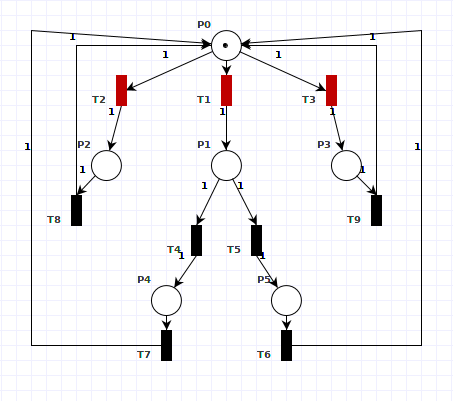
\includegraphics[width=\textwidth]{zad1_maszyna_stanow.png}
\caption{Schemat sieci}
\end{figure}

\begin{figure}[H]
\centering
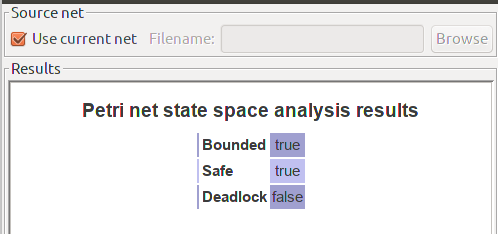
\includegraphics[width=\textwidth]{zad1_bounded_safe_deadlock.png}
\caption{Właściwości sieci}
\end{figure}

\begin{figure}[H]
\centering
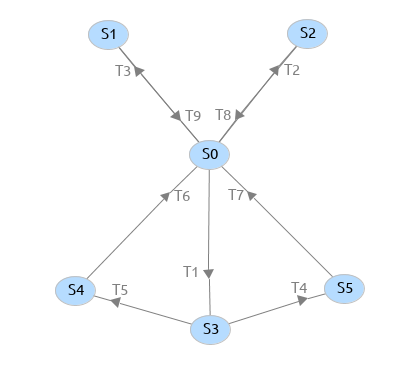
\includegraphics[width=\textwidth]{zad1_reachability_graph.png}
\caption{Graf osiągalności}
\end{figure}

Z grafu osiągalności możemy odczytać, że osiągalne znakowania to
\[ (0,0,0,0,0,1), (0,0,0,0,1,0), (0,0,0,1,0,0), (0,0,1,0,0,0), (0,1,0,0,0,0), (1,0,0,0,0,0) \]
W każdym znakowaniu liczba znaczników jest równa dokładnie 1. Sieć jest więc 1-ograniczona, czyli również bezpieczna. \\
Ponieważ dla każdego znakowania osiągalnego ze znakowania początkowego liczba znaczników jest stała to przedstawiona sieć jest zachowawcza. \\
Każde przejście jest przedstawione jako krawędź w grafie, więc ma szansę się wykonać. Z tego wniosek, że są one żywotne. \\
Ponieważ każde przejście jest żywotne i z każdego przejścia możemy wrócić do stanu początkowego, to wiemy, że sieć jest żywotna i nie są możliwe zakleszczenia.

\begin{figure}[H]
\centering
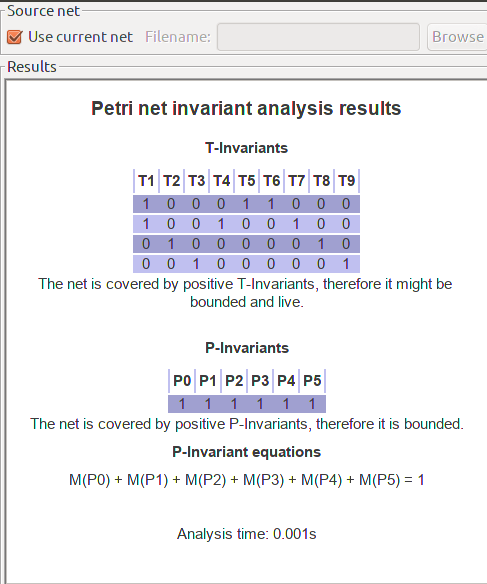
\includegraphics[width=\textwidth]{zad1_invariant_analisis.png}
\caption{Analiza niezmienników}
\end{figure}

Widzimy, że sieć jest odwracalna ponieważ w T-invariants pojawia się każdy możliwy stan. Każdy wiersz odpowiada jednej "pętli" od stanu początkowego do stanu początkowego. \\
P-invariants pokazuje nam zbiory stanów o stałej liczbie znaczników. Widzimy, że mamy tylko jeden taki zbiór zawierający wszystkie miejsca, więc nasza sieć jest na pewno ograniczona.

\section{Zadanie 2}
Narysowany w symulatorze przykład:

\begin{figure}[H]
\centering
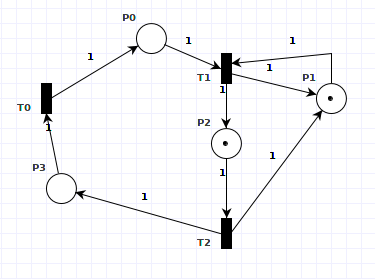
\includegraphics[width=\textwidth]{zad2_siec.png}
\caption{Schemat sieci}
\end{figure}


\begin{figure}[H]
\centering
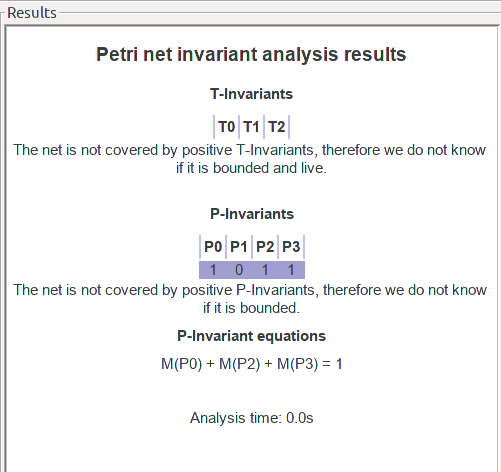
\includegraphics[width=\textwidth]{zad2_invariant_analysis.png}
\caption{Analiza niezmienników}
\end{figure}

Widzimy jeden niekompletny zbiór P-invariants. Możemy zauważyć, że w każdej pętli $T2\rightarrow T0 \rightarrow T1$ w stanie P1 pojawia się dodatkowy znacznik. Sieć nie jest odwracalna ani ograniczona, bo wraz z działaniem pojawiają się kolejne znaczniki i tak w nieskończoność bez możliwości ich usunięcia.

\begin{figure}[H]
\centering
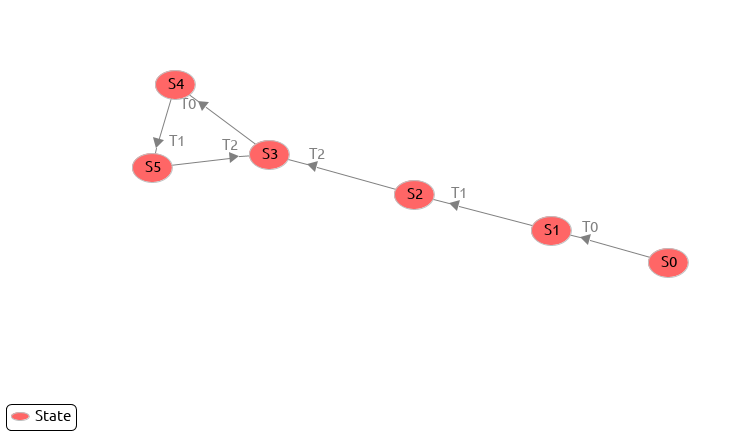
\includegraphics[width=\textwidth]{zad2_reachability_graph.png}
\caption{Graf osiągalności}
\end{figure}

%%%%% Tutaj napisać czy sieć jest żywa
Ponieważ stan $S4 = (1, \omega, 0, 0)$ gdzie $\lim \omega = \infty$, to sieć nie jest ograniczona.

\section{Zadanie 3}

\begin{figure}[H]
\centering
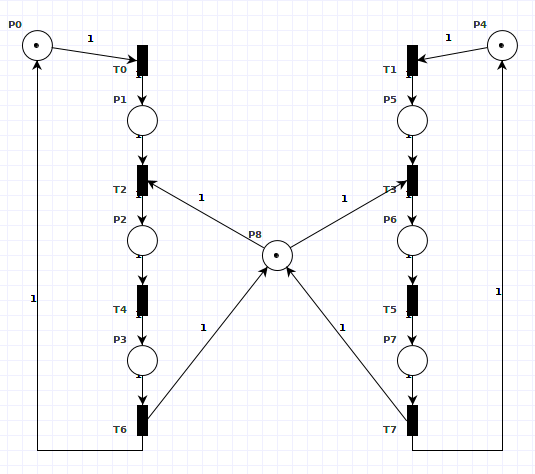
\includegraphics[width=\textwidth]{zad3_siec.png}
\caption{Schemat sieci}
\end{figure}

\begin{figure}[H]
\centering
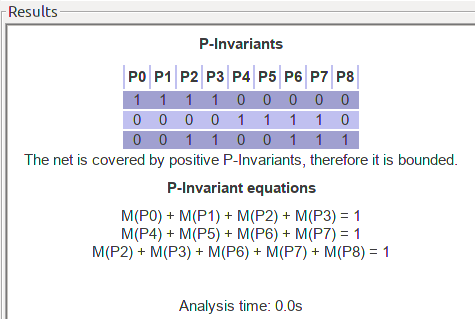
\includegraphics[width=\textwidth]{zad3_invariant_analysis.png}
\caption{Analiza niezmienników}
\end{figure}

\begin{equation}
    M(P0) + M(P1) + M(P2) + M(P3) = 1 \label{eq:3_1}
\end{equation}
\begin{equation}
    M(P4) + M(P5) + M(P6) + M(P7) = 1 \label{eq:3_2}
\end{equation}
\begin{equation}
    M(P2) + M(P3) + M(P6) + M(P7) + M(P8) = 1 \label{eq:3_3}
\end{equation}

Równanie \eqref{eq:3_1} odpowiada lewemu procesowi - krąży w nim stale jeden znacznik, stąd niezmiennik.
Podobnie z kolejnym równaniem. Równanie \eqref{eq:3_3} odpowiada sekcjom krytycznym obu procesów. Naraz nie mogą się tam pojawić dwa znaczniki.
Dlatego równanie to pokazuje poprawność ochrony sekcji krytycznej.

\section{Zadanie 4}

\begin{figure}[H]
\centering
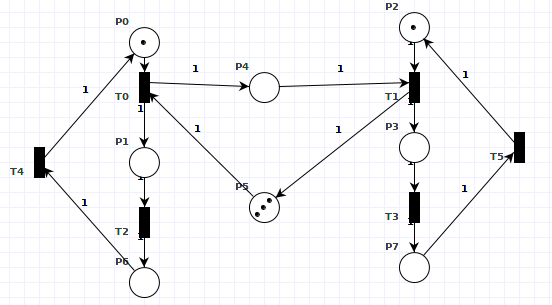
\includegraphics[width=\textwidth]{zad4_siec.png}
\caption{Schemat sieci}
\end{figure}

\begin{figure}[H]
\centering
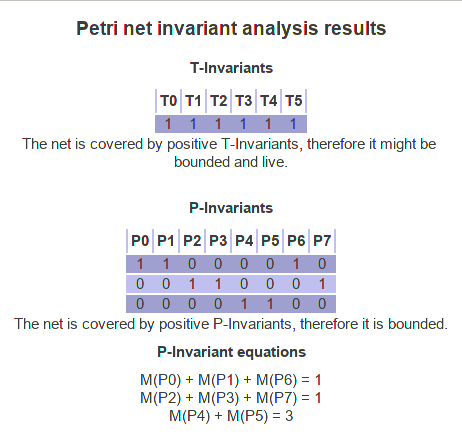
\includegraphics[width=0.7\textwidth]{zad4_invariant_analysis.png}
\caption{Analiza niezmienników}
\end{figure}

Możemy zauważyć, że mamy 3 rozłączne zbiory P-niezmienników, których suma stanowi całą sieć. Sieć jest zatem zachowawcza a dokładna ilość znaczników, które się w niej znajdują to suma prawych stron równań zapisanych wyżej. \\
Dokładny rozmiar bufora to suma rozmiaru bufora dla producenta i rozmiaru bufora dla konsumenta, czyli $M(P4) + M(P5) = 3$

\section{Zadanie 5}

\begin{figure}[H]
\centering
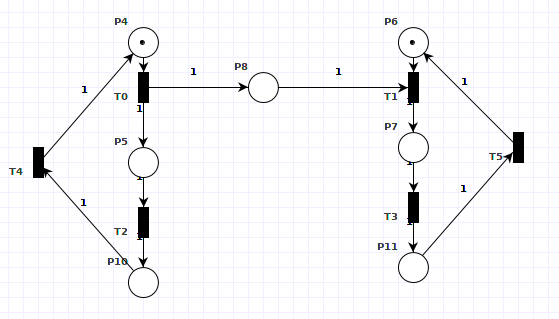
\includegraphics[width=\textwidth]{zad5_siec.png}
\caption{Schemat sieci}
\end{figure}

\begin{figure}[H]
\centering
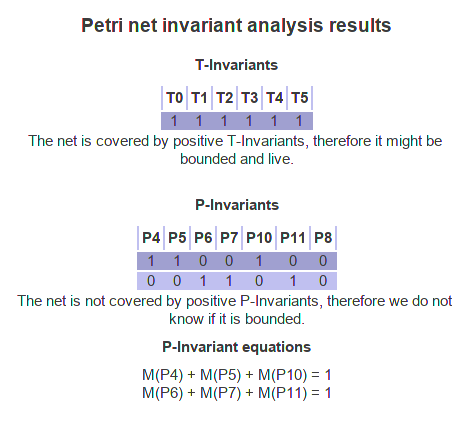
\includegraphics[width=0.7\textwidth]{zad5_invariant_analysis.png}
\caption{Analiza niezmienników}
\end{figure}

Widać, że nie mamy pokrycia miejsca P8, więc nie wiemy ile może się tam pojawić znaczników. Sieć nie jest zatem zachowawcza.

\section{Zadanie 6}

\begin{figure}[H]
\centering
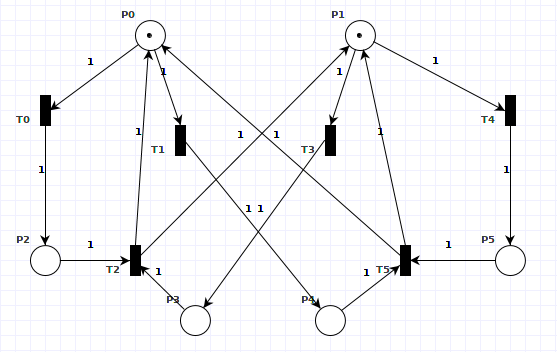
\includegraphics[width=\textwidth]{zad6_siec.png}
\caption{Schemat sieci}
\end{figure}

\begin{figure}[H]
\centering
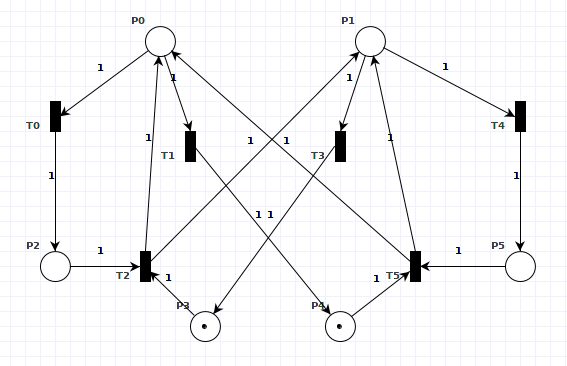
\includegraphics[width=\textwidth]{zad6_zakleszczenie.png}
\caption{Przykład zakleszczenia (po przejściach T1, T3)}
\end{figure}

\begin{figure}[H]
\centering
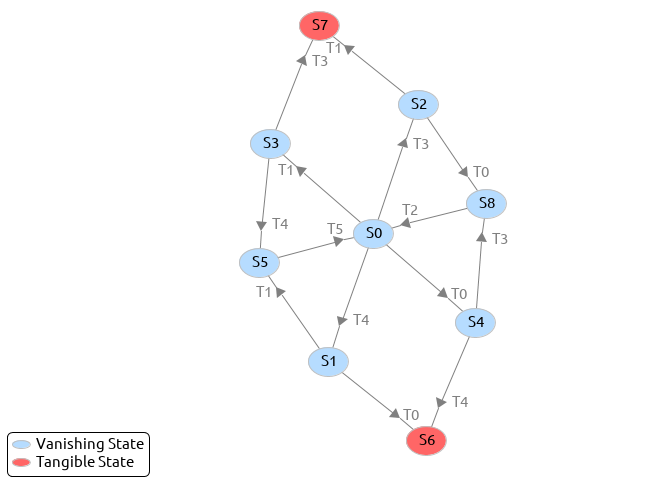
\includegraphics[width=\textwidth]{zad6_reachability_graph.png}
\caption{Graf przejść}
\end{figure}

Ze wszystkich wygenerowanych Tangible State odczytujemy znakowania, które doprowadzają do zakleszczenia. W naszym wypadku są to $(0,0,0,1,1,0)$ oraz $(0,0,1,0,0,1)$.

\begin{figure}[H]
\centering
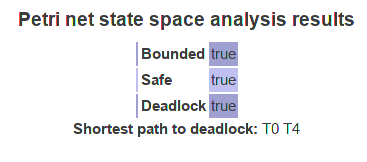
\includegraphics[width=0.65\textwidth]{zad6_state_space_analysis.png}
\caption{State Space Analysis}
\end{figure}
\end{document}

